\documentclass[a4paper,11pt]{article}
% ---- graphiques
\usepackage[pdftex]{graphicx}
\usepackage{wrapfig}
\usepackage{color}
%\usepackage{hyperref}

% for latex2html
\usepackage{html}

% for accents
\usepackage[latin1]{inputenc}
\usepackage[T1]{fontenc}

\usepackage{algorithm}
\usepackage{algorithmic}

\definecolor{darkgreen}{rgb}{0,0.4,0}
\definecolor{darkblue}{rgb}{0,0,0.4}
\definecolor{darkgray}{rgb}{0.2,0.2,0.2}

% ---- inclusion de codes
\usepackage{listings}
\lstset{showstringspaces=false,tabsize=4,basicstyle=\scriptsize\sffamily,breaklines=true,breakatwhitespace=true,framexleftmargin=5mm, frame=shadowbox, framesep=1pt,rulesepcolor=\color{darkgray},rulesep=.5pt,keywordstyle=\bf\color{blue},commentstyle=\color{magenta},stringstyle=\color{red},numbers=left,numberstyle=\tiny,numbersep=5pt,columns=flexible}

\lstdefinestyle{bash}{language=bash}
\lstdefinestyle{Perl}{language=Perl}
\lstdefinestyle{C++}{language=C++,emph={__global__,__shared__,__syncthreads,blockIdx,threadIdx,float3,float4},emphstyle=\bf\color{darkgreen}}
\lstdefinestyle{DTD}{language=XML}
\lstdefinestyle{XML}{language=XML,usekeywordsintag=false,markfirstintag=true}
%begin{latexonly}
\newcommand{\includecode}[2]{
\lstinputlisting[style=#1]{#2}
}
%end{latexonly}
\begin{htmlonly}
\newcommand{\includecode}[2]{  \htmladdnormallink{#2}{../../#2} }
\end{htmlonly}

%\lstnewenvironment{code}{}{}
\lstnewenvironment{code_bash}{\lstset{style=bash}}{}
\lstnewenvironment{code_perl}{\lstset{style=Perl}}{}
\lstnewenvironment{code_cpp}{\lstset{style=C++}}{}
\lstnewenvironment{code_dtd}{\lstset{style=DTD}}{}
\lstnewenvironment{code_xml}{\lstset{style=XML}}{}

\newcommand{\textcode}[1]{{\sf #1}}



%
\newcommand{\sofa}{SOFA}
\newcommand{\todo}[1]{}
\newcommand{\eg}{\textit{e.g.} }

\renewcommand{\vec}[1]{\ensuremath{\mathbf{#1 }}} % vector
\newcommand{\Vx}{\vec{x} } % position vector
\newcommand{\Vv}{\vec{v} } % velocity vector
\newcommand{\Va}{\vec{a} } % acceleration vector
\newcommand{\Vf}{\vec{f}} % force
\newcommand{\Vdv}{\vec{\delta\Vv}} % change of velocity vector (unknown in implicit CG, and used in constraint solver
\renewcommand{\P}{\mat{P} } % projection to a constrained space.

\newcommand{\JNL}{\mathbf{\mathcal{J}} }     % mapping des positions
\newcommand{\J}{\mat J }                 % mapping lineaire
\newcommand{\M}{\mat M }             % matrice de masse
\newcommand{\K}{\mat K }             % matrice de raideur
\newcommand{\B}{\mat B }             % matrice d'amortissement
\newcommand{\G}{\mat G }             % jacobien des contraintes



% ---- inclusion de codes
\definecolor{darkgreen}{rgb}{0,0.4,0}
\definecolor{darkblue}{rgb}{0,0,0.4}
\definecolor{darkgray}{rgb}{0.2,0.2,0.2}


% macros mathematiques
\newcommand{\ma}[1]{\ensuremath{\mathbf {#1}}}
\newcommand{\ve}[1]{\ensuremath{\mathbf {#1}}}

\usepackage{amsmath}
\usepackage{amsfonts}
\usepackage{amssymb}

% character styles
\newcommand{\bm}[1]{\ensuremath{\mathbf{{#1}}}}
\newcommand{\mcal}[1]{\mbox{$\mathcal #1$}} % rondes math
\newcommand{\bmcal}[1]{\mbox{\boldmath $\mathcal #1$}} % rondes grasses math
\newcommand{\ensemble}[1]{\mbox{$\mathbb{#1}$}}
\newcommand{\RRR}{\mbox{$\ensemble{R}^3$}} 


 % This file is in parent directory. Your TEXINPUTS environment variable must include .. to reach this file. Example: setenv TEXINPUTS ..:../..:${TEXINPUTS}

% ---- format de page A4
	\setlength{\textwidth }{16cm}	% largeur de ligne
	\setlength{\textheight}{23cm}   % hauteur du texte
	\setlength{\oddsidemargin}{0cm} % marge pages impaires
	\setlength{\evensidemargin}{0cm}% marge pages paires
	\setlength{\topmargin}{0cm} 	
	\setlength{\headheight}{14pt} 
	\setlength{\headsep}{0.5cm} 


% Title Page
\title{Non Uniform Mechanical Properties for Hexahedron FEM}
\author{The \sofa{} team (Matthieu Nesme - matthieu.nesme@imag.fr)}
\date{2008}

\makeindex
\begin{document} 
\maketitle

\begin{abstract}
This document explains how using the NonUniformHexahedronFEMForceFieldAndMass that permits to animate a mesh embedded into a coarse mechanical grid by taking into account matter distribution into element.
\\It implements the article

\begin{verbatim}
      @InProceedings{NPF06,
      author       = "Nesme, Matthieu and Payan, Yohan and Faure, Fran\c{c}ois",
      title        = "Animating Shapes at Arbitrary Resolution with Non-Uniform Stiffness",
      booktitle    = "Eurographics Workshop in Virtual Reality Interaction and Physical Simulation (VRIPHYS)",
      month        = "nov",
      year         = "2006",
      organization = "Eurographics",
      address      = "Madrid",
      url          = "http://www-evasion.imag.fr/Publications/2006/NPF06"}
 \end{verbatim}
 
\end{abstract}

\tableofcontents
\newpage
\subsection{NonUniformHexahedronFEMForceFieldAndMass}
\graphicspath{{../modules/}}  % to include images


\subsubsection{Concepts}

This force field implement the article :

\begin{verbatim}
      @InProceedings{NPF06,
      author       = "Nesme, Matthieu and Payan, Yohan and Faure, Fran\c{c}ois",
      title        = "Animating Shapes at Arbitrary Resolution with Non-Uniform Stiffness",
      booktitle    = "Eurographics Workshop in Virtual Reality Interaction and Physical Simulation (VRIPHYS)",
      month        = "nov",
      year         = "2006",
      organization = "Eurographics",
      address      = "Madrid",
      url          = "http://www-evasion.imag.fr/Publications/2006/NPF06"}
 \end{verbatim}
 
 
 
The basic idea, illustrated in figure \ref{fig:condensation}, is :


\begin{figure}
\begin{center}
	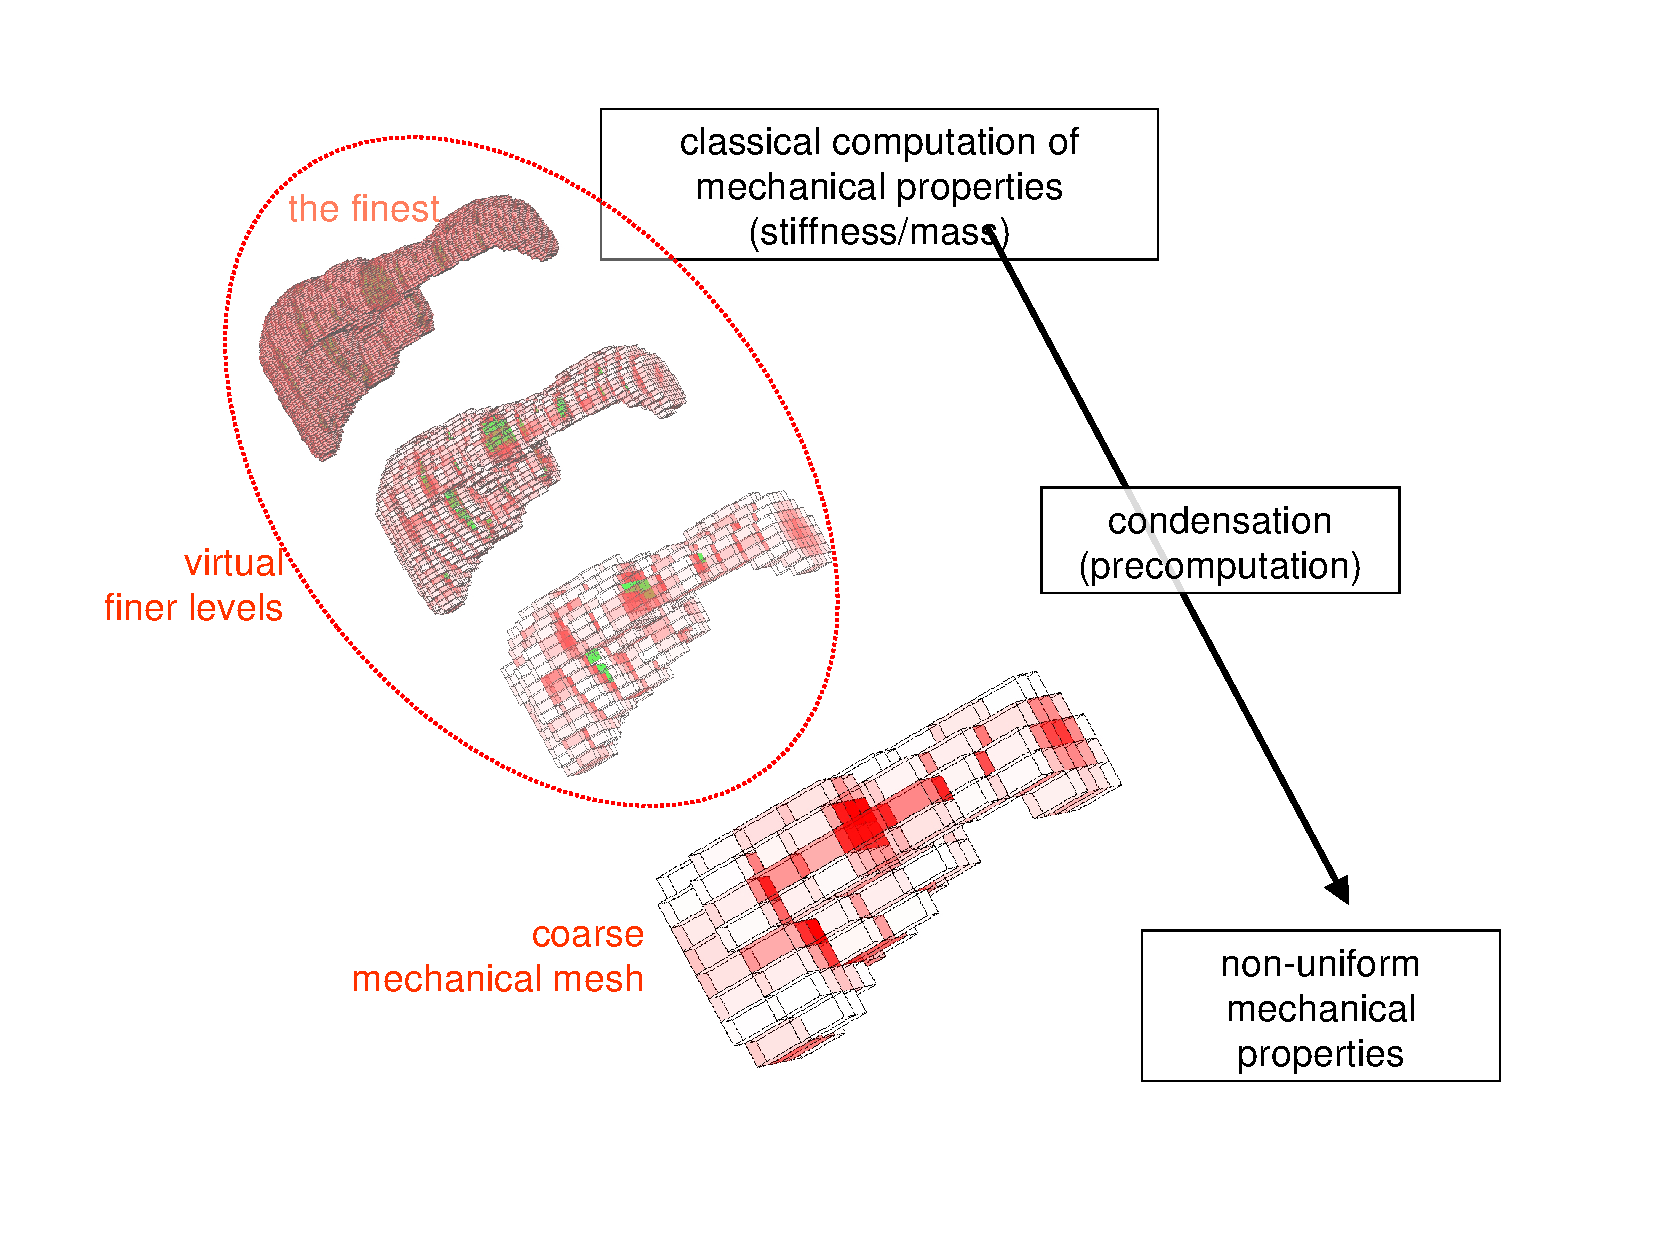
\includegraphics[width=\linewidth]{forcefield/nonUniformHexahedron/condensation.pdf}
\end{center}
	\caption{The condensation principle.}
	\label{fig:condensation}
\end{figure}



\begin{itemize}
\item the use of finer virtual levels of SparseGrid
\item the computation of classical mechanical matrices (mass and stiffness) at the finest resolution and the condensation of theses matrices to the current coarse mechanical resolution
\end{itemize}


\textbf{Warning} : actually the NonUniformHexahedronFEMForceFieldAndMass is only working with SparseGridTopology, and need enough finer virtual levels to compute the condensation. 

\subsubsection{Data Fields}

\begin{itemize}
\item From HexahedronFEMForceFieldAndMass
	\begin{itemize}
	\item method (char) : large/polar, the corotationnal method (default = large)
	\item poissonRatio, youngModulus, density (float) : mechanical properties (density = volumetric mass in english $kg.m^{-3}$)
	\item assembling (bool) : assembling the global system matrix ? (default = false)
	\end{itemize}
\item Specific to NonUniformHexahedronFEMForceFieldAndMass
	\begin{itemize}
	\item nbVirtualFinerLevels (int) : how many finer virtual levels are employed in the condensation stage ? (default = 0)
	\end{itemize}
\item A hack on masses (for debugging)
		\begin{itemize}
	\item useMass (bool) : are the condensated mass matrices are used ? (if not, scalar masses concentrated on particles are used) (default = 0)
	\item totalMass (float) : if useMass=false, the scalar mass of the object
	\end{itemize}
\end{itemize}


\subsubsection{Example}



\begin{verbatim}

<Node name="non uniform">
   <Object type="SparseGrid"
                   n="4 4 4"
                   filename="mesh/mymesh.obj"
                   nbVirtualFinerLevels="2"  />
   <Object type="MechanicalObject"/>
   <Object type="NonUniformHexahedronFEMForceFieldAndMass"
                   nbVirtualFinerLevels="2"
                   youngModulus="20000"
                   poissonRatio="0.3"
                   density="10" />
</Node>

\end{verbatim}

\textbf{Important} : note that the SparseGrid has nbVirtualFinerLevels=2 in order to built enough finer virtual levels. This SparseGrid$->$nbVirtualFinerLevels has to be greater or equal to the NonUniformHexahedronFEMForceFieldAndMass$->$nbVirtualFinerLevels.
\\

A more complex example can be found in : examples/Components/forcefield/NonUniformHexahedronFEMForceFieldAndMass.scn where a comparison with a classical HexahedronFEMForceFieldAndMassForceField is done.




\end{document}

